\subsection{Requisitos de la aplicación}

Este apartado describe los requisitos esenciales que deben cumplirse para el correcto funcionamiento de la aplicación web propuesta. Los requisitos funcionales especifican las principales características que permitirán la gestión de entidades en el AD, mientras que los requisitos no funcionales establecen criterios relacionados con el rendimiento, la seguridad y la usabilidad del sistema. Además, se incluye un diagrama de caso de uso para ilustrar la interacción de los usuarios con las funcionalidades clave del sistema.

\subsubsection{Casos de uso del sistema}

Los casos de uso del sistema representan las interacciones entre los actores y las funcionalidades clave de la aplicación. A través de estos, se detallan los escenarios en los que los usuarios, administradores y otros actores relevantes interactúan con el sistema para cumplir con los objetivos propuestos. A continuación en la \autoref{fig:system-use-cases-diagram}, se presenta un diagrama de caso de uso que proporciona una vista general de las acciones que los usuarios pueden realizar, contribuyendo a una mejor comprensión de los requisitos funcionales definidos.

\begin{figure}[H]
    \centering
    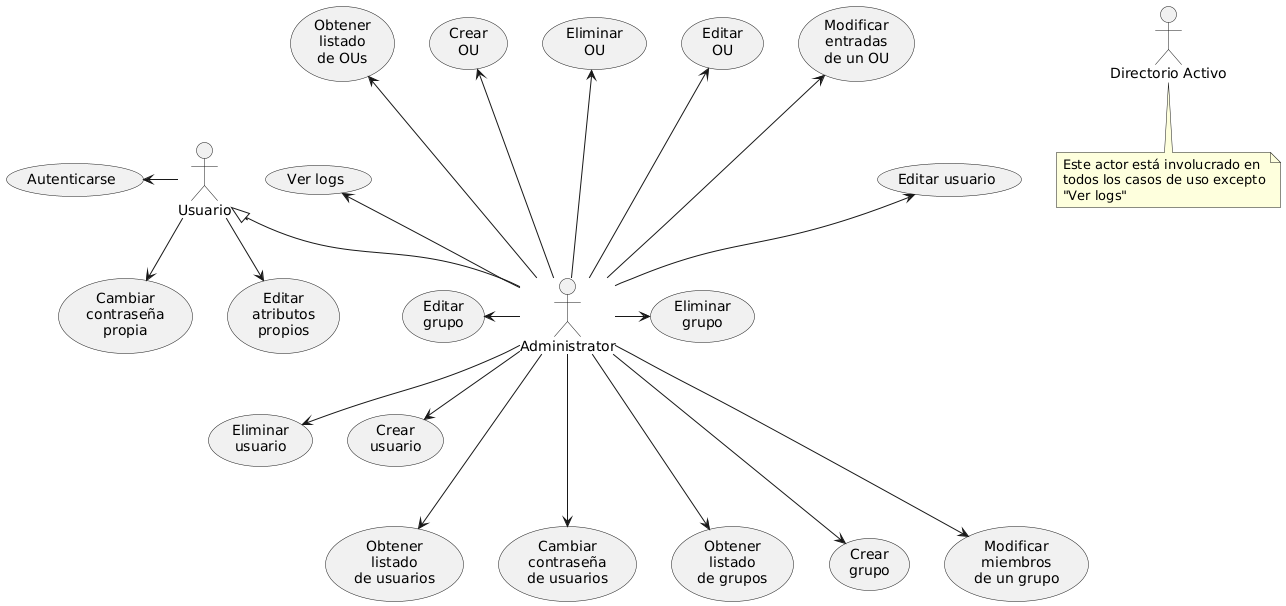
\includegraphics[width=\linewidth]{images/puml/system-diagram/system-diagram.png}
    \caption{Diagrama de casos de uso del sistema}
    \label{fig:system-use-cases-diagram}
\end{figure}
\subsubsection{Requisitos funcionales}

Los requisitos funcionales definen las funcionalidades y comportamientos que la aplicación debe ofrecer para cumplir con las necesidades del usuario y los objetivos del proyecto. En la \autoref{table:functional-requirements} a continuación se desglosan los requisitos funcionales del sistema.



\begin{longtable}{|l|p{5cm}|p{8.5cm}|}
    \caption{Requisitos funcionales del sistema}
    \label{table:functional-requirements}                                                                                                                                                                                          \\
    \hline
    \textbf{Código} & \textbf{Requisito}                                                              & \textbf{Descripción}                                                                                                       \\
    \hline
    \endfirsthead
    \textbf{RF1}   & Gestión de Usuarios: Creación de usuarios                                       & La aplicación debe permitir la creación de nuevas cuentas de usuario en el AD.                                             \\ \hline
    \textbf{RF2}   & Gestión de Usuarios: Modificación de usuarios                                   & Los administradores deben poder actualizar la información de los usuarios, como nombres, correos electrónicos, roles, etc. \\ \hline
    \textbf{RF3}   & Gestión de Usuarios: Eliminación de usuarios                                    & La aplicación debe permitir la eliminación segura de cuentas de usuario.                                                   \\ \hline
    \textbf{RF4}   & Gestión de Usuarios: Asignación de roles y permisos                             & Debe ser posible asignar y modificar roles y permisos a los usuarios para definir su nivel de acceso a los recursos.       \\ \hline
    \textbf{RF5}   & Gestión de Grupos: Creación de grupos                                           & Permitir la creación de nuevos grupos en el AD.                                                                            \\ \hline
    \textbf{RF6}   & Gestión de Grupos: Modificación de grupos                                       & Posibilidad de añadir o remover usuarios de grupos existentes.                                                             \\ \hline
    \textbf{RF7}   & Gestión de Grupos: Eliminación de grupos                                        & Permitir la eliminación de grupos.                                                                                         \\ \hline
    \textbf{RF8}   & Gestión de Unidades Organizacionales (OU): Creación de OU                       & La aplicación debe permitir la creación de nuevas Unidades Organizacionales dentro del AD.                                 \\ \hline
    \textbf{RF9}   & Gestión de Unidades Organizacionales (OU): Modificación de OU                   & Los administradores deben poder renombrar y mover OUs dentro de la jerarquía del directorio.                               \\ \hline
    \textbf{RF10}  & Gestión de Unidades Organizacionales (OU): Eliminación de OU                    & Debe ser posible eliminar OUse.                                                                                            \\ \hline
    \textbf{RF11}  & Gestión de Unidades Organizacionales (OU): Asignación de usuarios y grupos a OU & La aplicación debe facilitar la asignación de usuarios y grupos a las OUs para una mejor organización dentro del AD.       \\ \hline
    \textbf{RF12}  & Autenticación y Autorización: Integración con LDAP                              & La aplicación debe autenticarse a través de LDAP con el AD para validar usuarios y permisos.                               \\ \hline
    \textbf{RF13}  & Autenticación y Autorización: Gestión de sesiones                               & Manejo de sesiones de usuario con opciones de inicio y cierre de sesión seguro.                                            \\ \hline
    \textbf{RF14}  & Auditoría y Registro de Actividades: Registro de eventos                        & La aplicación debe registrar todas las operaciones realizadas sobre los usuarios, grupos y OUs, incluyendo quién y cuándo. \\ \hline
    \textbf{RF15}  & Interfaz de Usuario (UI): Consola de administración                             & Proveer una interfaz amigable y accesible para la gestión de usuarios, grupos, OUs y revisión del registro de eventos.     \\ \hline
    \textbf{RF16}  & Interfaz de Usuario (UI): Notificaciones                                        & Mostrar notificaciones en la UI para confirmar la ejecución exitosa de acciones o para advertir sobre errores.             \\ \hline
    \textbf{RF17}  & Configuración de la Aplicación: Facilidad de configuración                      & La aplicación debe ser fácilmente configurable a través de archivos .json o .yaml, validados mediante JSON Schema.         \\ \hline
\end{longtable}

\subsubsection{Requisitos no funcionales}

Los requisitos no funcionales describen las cualidades que debe tener la aplicación para garantizar un desempeño óptimo y satisfacer las expectativas de los usuarios. En la \autoref{table:non-functional-requirements} se enumeran los requisitos funcionales que debe presentar el sistema.


\begin{longtable}{|l|l|p{12cm}|}
    \caption{Requisitos no funcionales del sistema}
    \label{table:non-functional-requirements}                                                                                                                                                 \\
    \hline
    \textbf{Código} & \textbf{Requisito} & \textbf{Descripción}                                                                                                                               \\
    \hline
    \endfirsthead
    \textbf{RNF1}   & Calidad            & La aplicación debe ser capaz de manejar un creciente número de usuarios y grupos sin degradación significativa en el rendimiento.                  \\ \hline
    \textbf{RNF2}   & Restricción        & La aplicación debe implementar mecanismos de seguridad como cifrado de datos, autenticación segura, y control de acceso basado en roles (RBAC).    \\ \hline
    \textbf{RNF3}   & Calidad            & Las operaciones críticas como la autenticación y la gestión de usuarios deben completarse en menos de 2 segundos en condiciones normales de carga. \\ \hline
    \textbf{RNF4}   & Calidad            & La interfaz debe ser intuitiva y fácil de usar, con una curva de aprendizaje mínima para administradores y usuarios avanzados.                     \\ \hline
    \textbf{RNF5}   & Restricción        & La aplicación debe ser compatible con múltiples navegadores web modernos y adaptarse a diferentes tamaños de pantalla (responsive design).         \\ \hline
    \textbf{RNF6}   & Calidad            & El código debe ser modular y bien documentado, facilitando futuras actualizaciones y correcciones de errores.                                      \\ \hline
    \textbf{RNF7}   & Calidad            & La configuración de la aplicación debe estar documentada de manera clara y accesible, disponible en línea en el sitio web del proyecto.            \\ \hline
    \textbf{RNF8}   & Restricción        & La aplicación debe ser web                                                                                                                         \\ \hline
    \textbf{RNF9}   & Restricción        & La aplicacion debe ser de código abierto                                                                                                           \\ \hline
\end{longtable}

